\section{Evaluation and Analysis}
In this section, we evaluate the above techniques to leverage the approximation-tolerance of the neural network to accelerate distributed training. We essentially perform \textit{training update elisions}, which involves not updating the weights and biases of specific layers at certain training steps. Two kinds of training elisions were explored:
\begin{itemize}
	\item \textit{Periodic Training Elision} involves performing training elisions once every $n$ steps, where $n$ is called the periodic elision interval. The parameters of the entire network are updated for $n-1$ steps, followed by a step where only parameters corresponding to certain layers are updated.
	\item \textit{Selective Early Termination} involves training the entire network until a given training step $\kappa$. For steps after $\kappa$, only parameters corresponding to certain layers are updated, while updates and gradient computation for other layers are elided.

\end{itemize}

Both types of approximations partially update the model weights in a specified training step. We expect that using update elision will reduce the amount of computation required in a training step, as well as the communication overhead required for distributed training. 

We now discuss the experimental results. Different approximation techniques are compared on the basis of classification accuracy (on the full testing data) and training time. We present results for both single node training as well as distributed training for a number of different cluster configurations. In each of our experiments, we checkpoint the model every 1000 trained steps, and use the checkpointed model to compute the achieved classification accuracy.

\subsection{Periodic Training Elision}
\subsubsection{Sensitivity of Different Layers to Training Elision}
To determine how the convergence of the model is impacted by the training elision for different layers, we conducted an experiment where we did not train or update a different number of layers every \emph{alternate step}. Figure~\ref{fig:fig1} depicts the accuracy achieved during training while periodically eliding training for a different number of layers starting from the bottom up (dashed lines) and top down (unbroken lines). 
\begin{figure}[t]
	\centering
	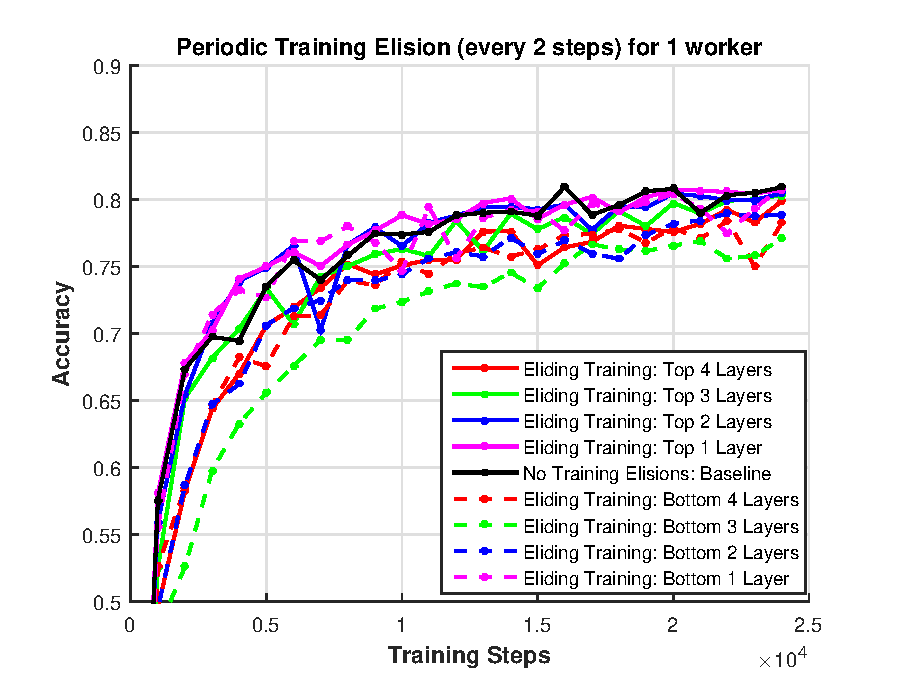
\includegraphics[width=0.8\columnwidth]{figures/fig1.eps}
	\caption{Periodic Training Elision (every 2 steps)}
	\label{fig:fig1}
\end{figure}
From Figure 1, we make the following observations: 
\begin{enumerate}
\item Eliding a single layer (top-most or bottom-most) has negligible impact on accuracy.
\item When eliding the \emph{same number} of layers, eliding training for the \emph{top layers} first consistently faster convergence and better accuracy than eliding the bottom layers.
\item Eliding the bottom 4 layers anomalously produces faster convergence than eliding the 3 bottom layers. 
\end{enumerate}
\subsubsection{Single Node Accuracy \& Training Time.}
In addition to Figure~\ref{fig:fig2} where the periodicity of training elision was \emph{two steps}, we conduct an experiment where we elide training at a periodicity of \emph{5 steps}. The accuracy results are depicted in Figure~\ref{fig:fig2}. We find that the neural network is resilient enough to tolerate this approximation irrespective of the number of layers for which training was elided with the exception of eliding the bottom 4 layers which produced a minor reduction in the accuracy. 
\begin{figure}[t]
	\centering
	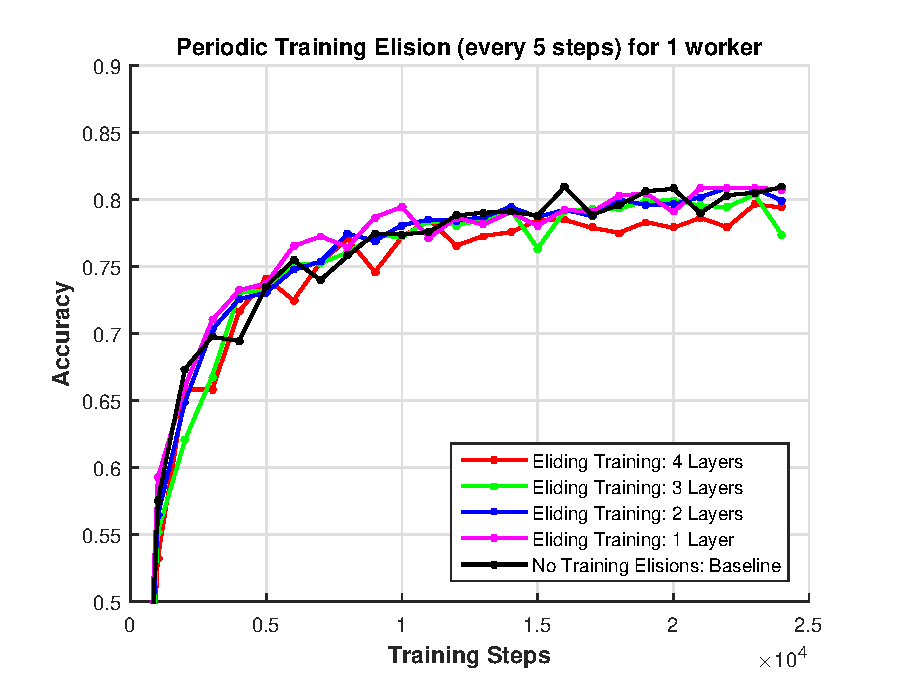
\includegraphics[width=0.8\columnwidth]{figures/fig2.eps}
	\caption{Periodic Training Elision (every 5 steps)}
	\label{fig:fig2}
\end{figure}
We also evaluated the resulting speedup in training time as a result of the described approximations. Figure~\ref{fig:fig3}depicts the normalized training speedup for both 2 and 5 step periodic training elision. We make the following observations: \emph{(i)} we observe that eliding training for 4 layers (2 step) produces a speedup of as much as 45\%; \emph{(ii)} Eliding training with a lower periodicity of 5 steps does not produce a significant bump in speedup (only 11.8\%); \emph{(iii)} Eliding a single layer produces only an insignificant improvement in training time. Since this is a single node experiment, the speedups come from eliding the gradient computation for several layers.  

\begin{figure}[t]
	\centering
	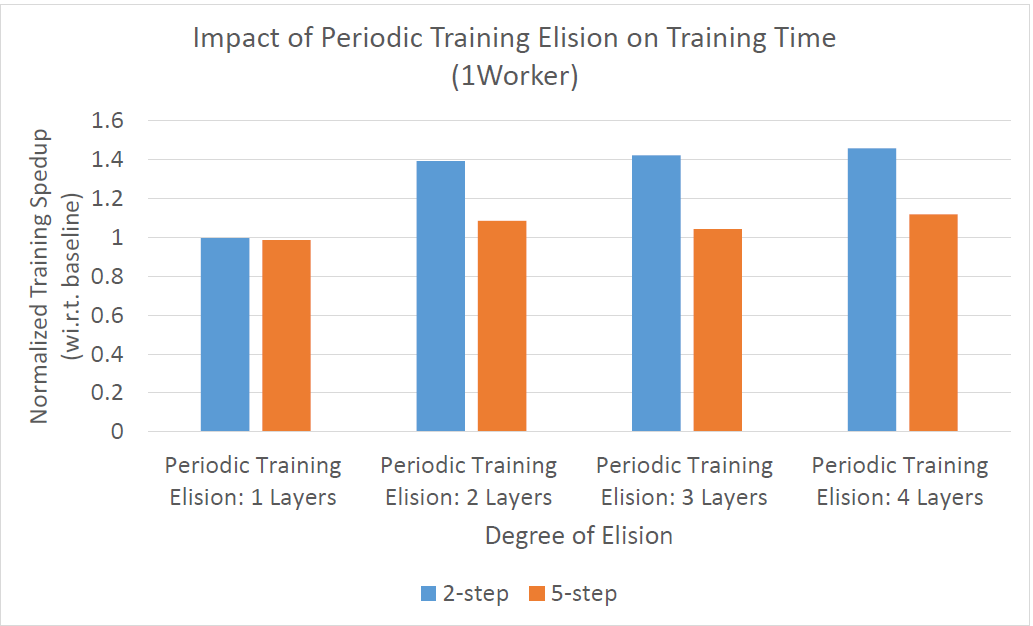
\includegraphics[width=0.8\columnwidth]{figures/fig3.PNG}
	\caption{Normalized speedup for Periodic Training Elision (every 2 and 5 steps)}
	\label{fig:fig3}
\end{figure}

%Figure 1: Periodic Training Elision (every 2 steps for both upper layers and lower layers) -- Accuracy
%Figure 2: Periodic Training Elision (every 5) -- Accuracy
%Figure 3: Periodic Training Elision (every 2 \& 5 steps for both upper layers and lower layers) -- Execution Time
\subsubsection{Mutiple Workers Accuracy and Training Time.}
Figure~\ref{fig:fig4} depicts periodic training elision in a distributed setting with 4 workers. We find that approximating training for both 3 and 4 layers does not have a noticeable impact on convergence or accuracy.\footnote{It is possible that the impact of approximation is only noticeable after our evaluated training time of 2000 steps.} Figure~\ref{fig:fig5} depicts the normalized speedup for periodic training elision with 4 workers. We find that periodic training elision is able to provide a speedup of as much as 2.7x while eliding training for 3 layers, and 2.85x for 4 layers. 

\begin{figure}[t]
	\centering
	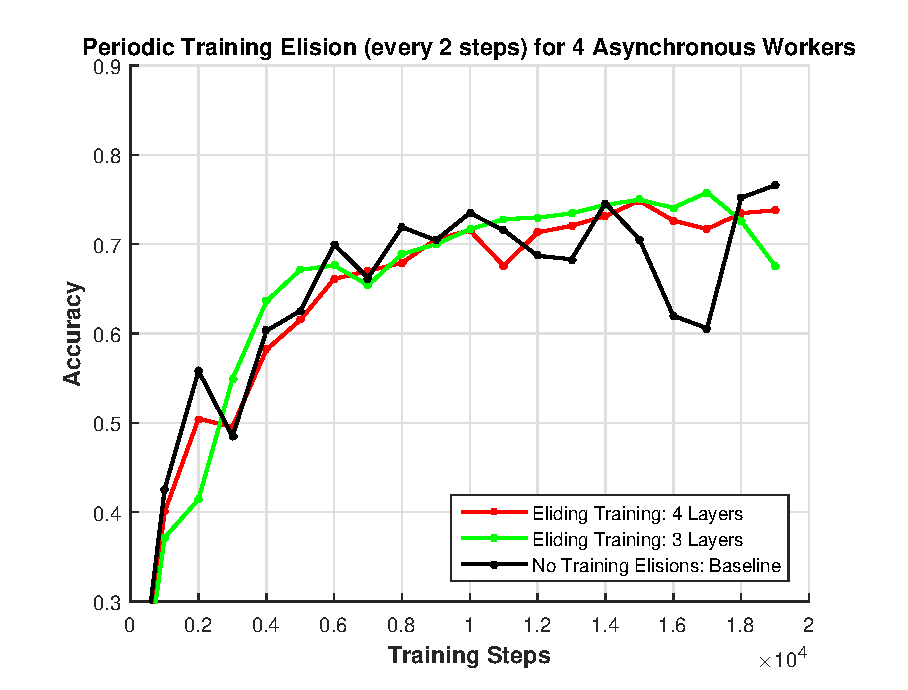
\includegraphics[width=0.8\columnwidth]{figures/fig4.eps}
	\caption{Periodic Training Elision: 4 workers (every 2 steps)}
	\label{fig:fig4}
\end{figure}

\begin{figure}[t]
	\centering
	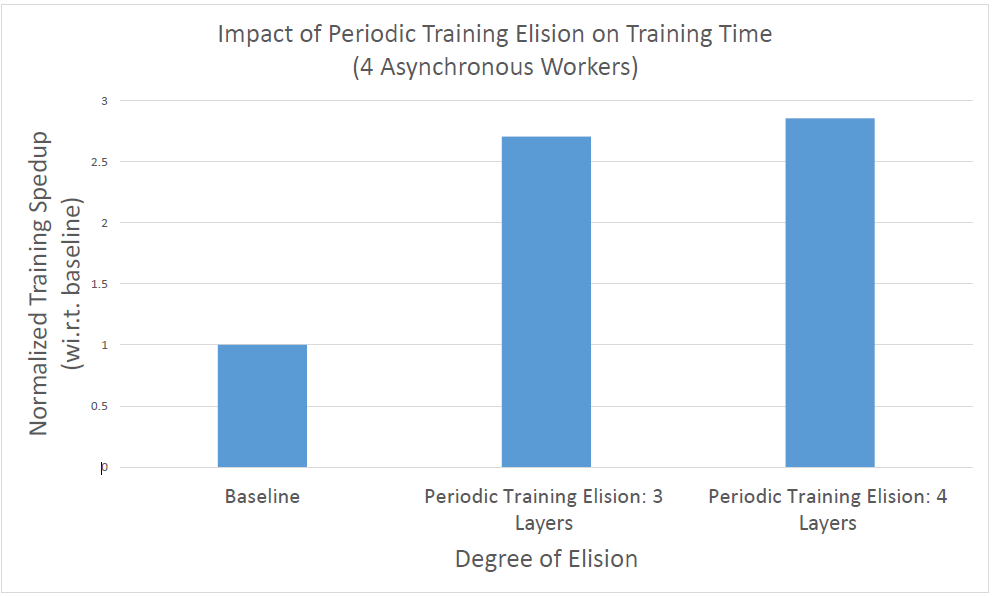
\includegraphics[width=0.8\columnwidth]{figures/fig5.PNG}
	\caption{Normalized speedup for Periodic Training Elision: 4 workers (every 2 steps)}
	\label{fig:fig5}
\end{figure}
%Figure 4: Periodic Training Elision 4 workers (every 2 steps for both upper layers and lower layers) -- Accuracy
%Figure 5: Periodic Training Elision 4 workers (every 2 steps for both upper layers and lower layers) -- Execution Time
\subsection{Selective Early Termination}
\subsubsection{Single Node Accuracy and Speedup} 
In Figure~\ref{fig:fig6}, we plot the obtained accuracy versus the training step for a selective early termination experiment running on a single machine. For each of the compared experiments we train all layers of the model until the 5000th training step. For the subsequent steps the training data is used to update only the top $\eta$ trainable layers of the model, where $\eta$ was chosen between $1$ to $4$ in our experiments. Note that, for a $N$ layer neural network $\eta=i$ corresponds to update elision for the first $N-\eta$ trainable layers. From the plot we can observe that eliding one layer has a neglible impact on accuracy, but eliding more than one layer leads to about 3\% drop in accuracy. After the training termination point, the network continues to improve accuracy for a short while, before converging on accuracy that is less than Baseline. 
Figure~\ref{fig:fig7} depicts the normalized speedup for selective early termination. We find that on a single machine selective early termination is able to produce as much as 2.3x reduction in training time.  

\begin{figure}[t]
	\centering
	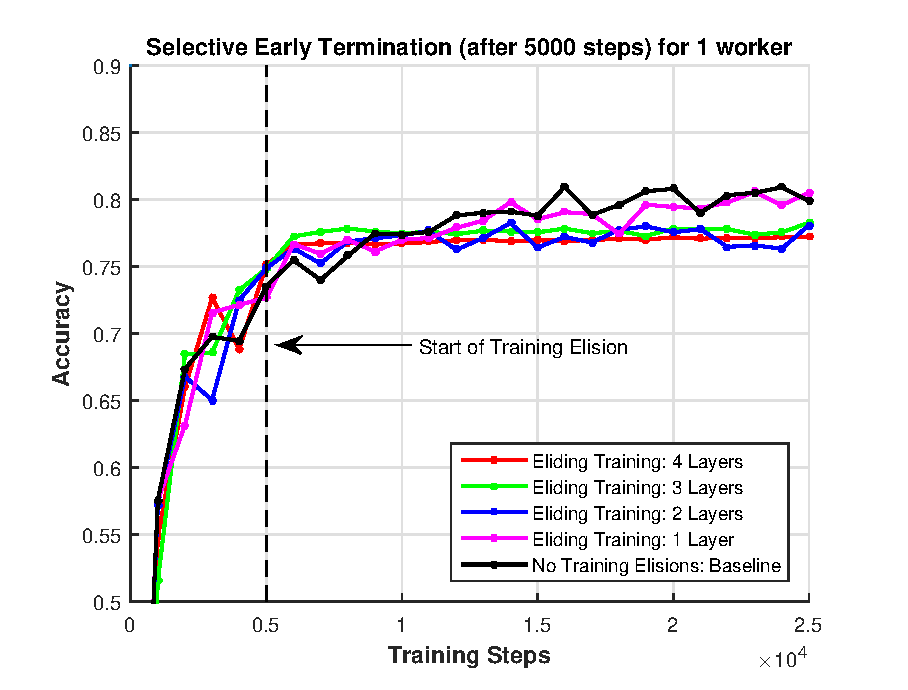
\includegraphics[width=0.8\columnwidth]{figures/fig6.eps}
	\caption{Selective Early Termination: 1 worker}
	\label{fig:fig6}
\end{figure}

\begin{figure}[t]
	\centering
	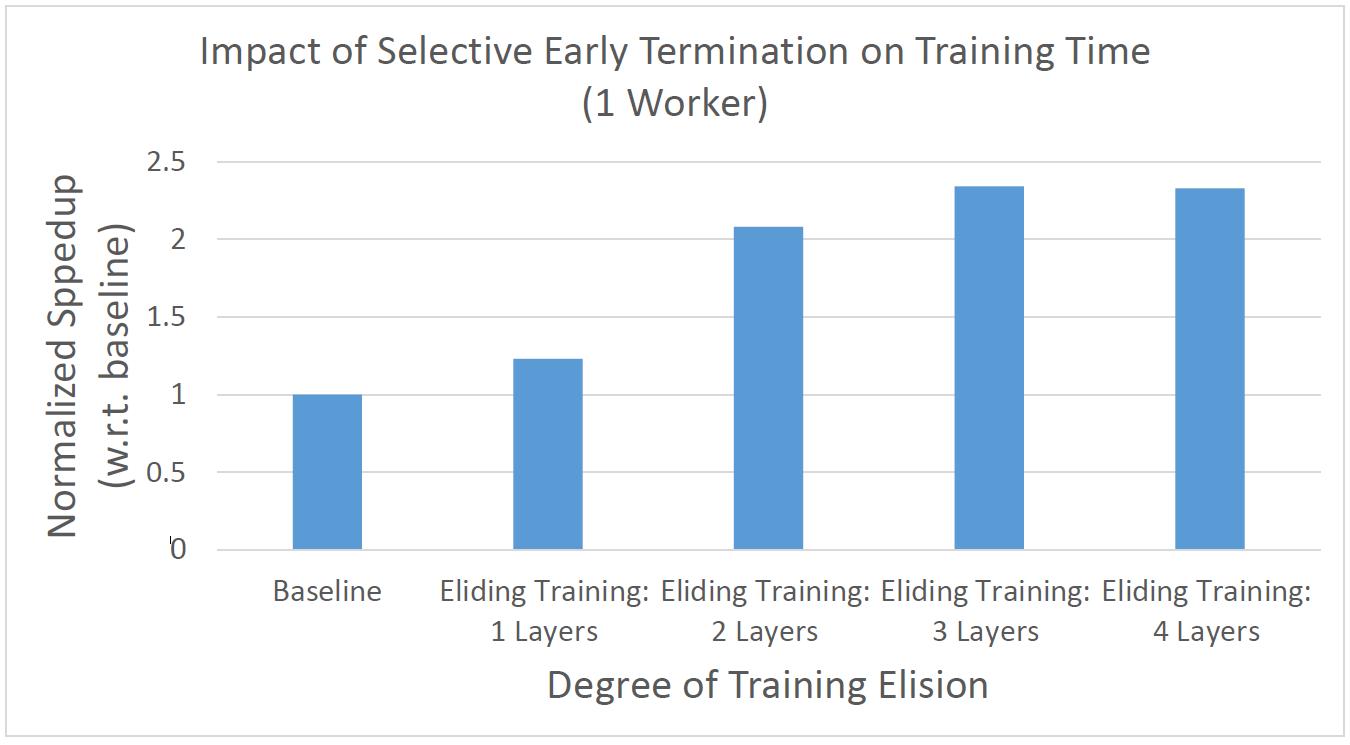
\includegraphics[width=0.8\columnwidth]{figures/fig7.PNG}
	\caption{Normalized speedup for Selective Early Termination: 1 worker}
	\label{fig:fig7}
\end{figure}
%Figure 6: Selective Early Termination (5K steps) -- Accuracy
%Figure 7: Selective Early Termination (5K steps) -- Execution Time
\subsubsection{Multiple Workers Accuracy and Speedups}

\begin{figure}[t]
	\centering
	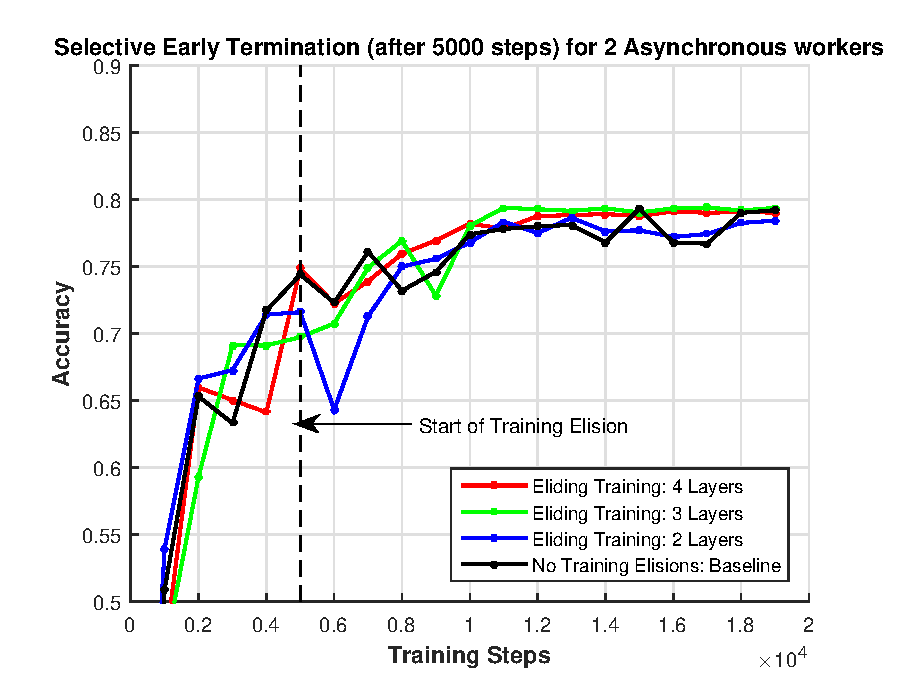
\includegraphics[width=0.8\columnwidth]{figures/fig8.eps}
	\caption{Selective Early Termination for 2 workers (after 5K steps)}
	\label{fig:fig8}
\end{figure}
\begin{figure}[t]
	\centering
	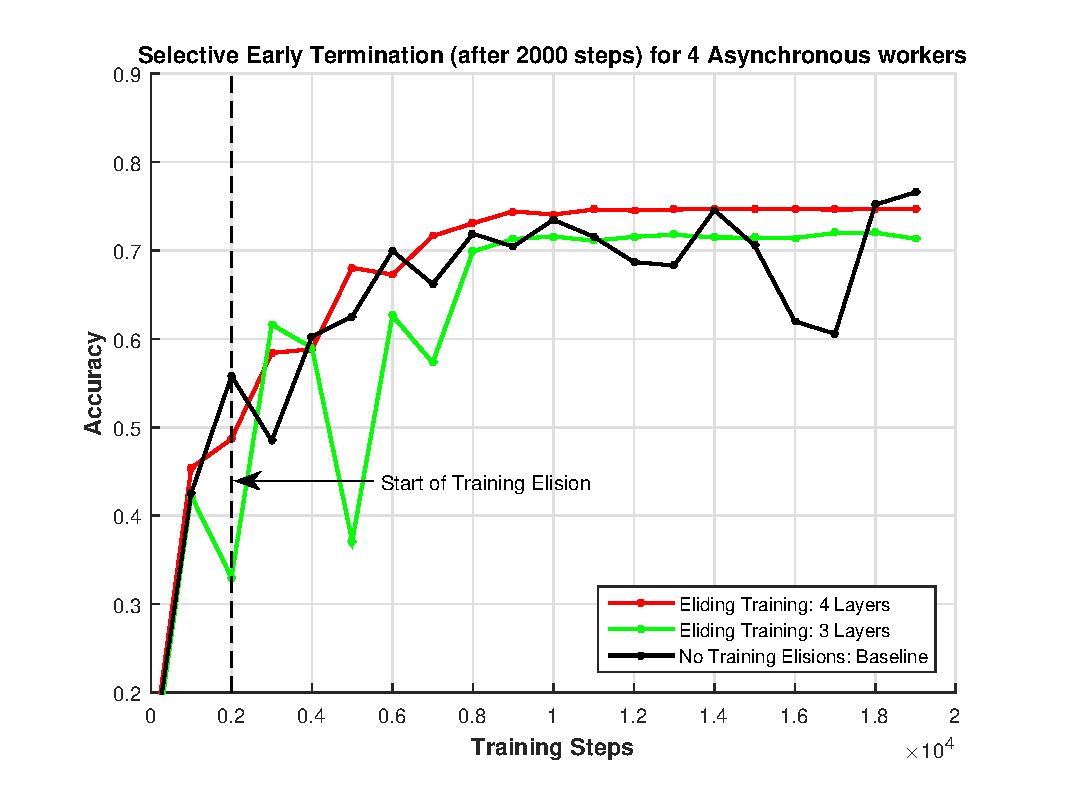
\includegraphics[width=0.8\columnwidth]{figures/fig9.eps}
	\caption{Selective Early Termination for 4 workers (after 2K steps)}
	\label{fig:fig9}
\end{figure}
\begin{figure}[t]
	\centering
	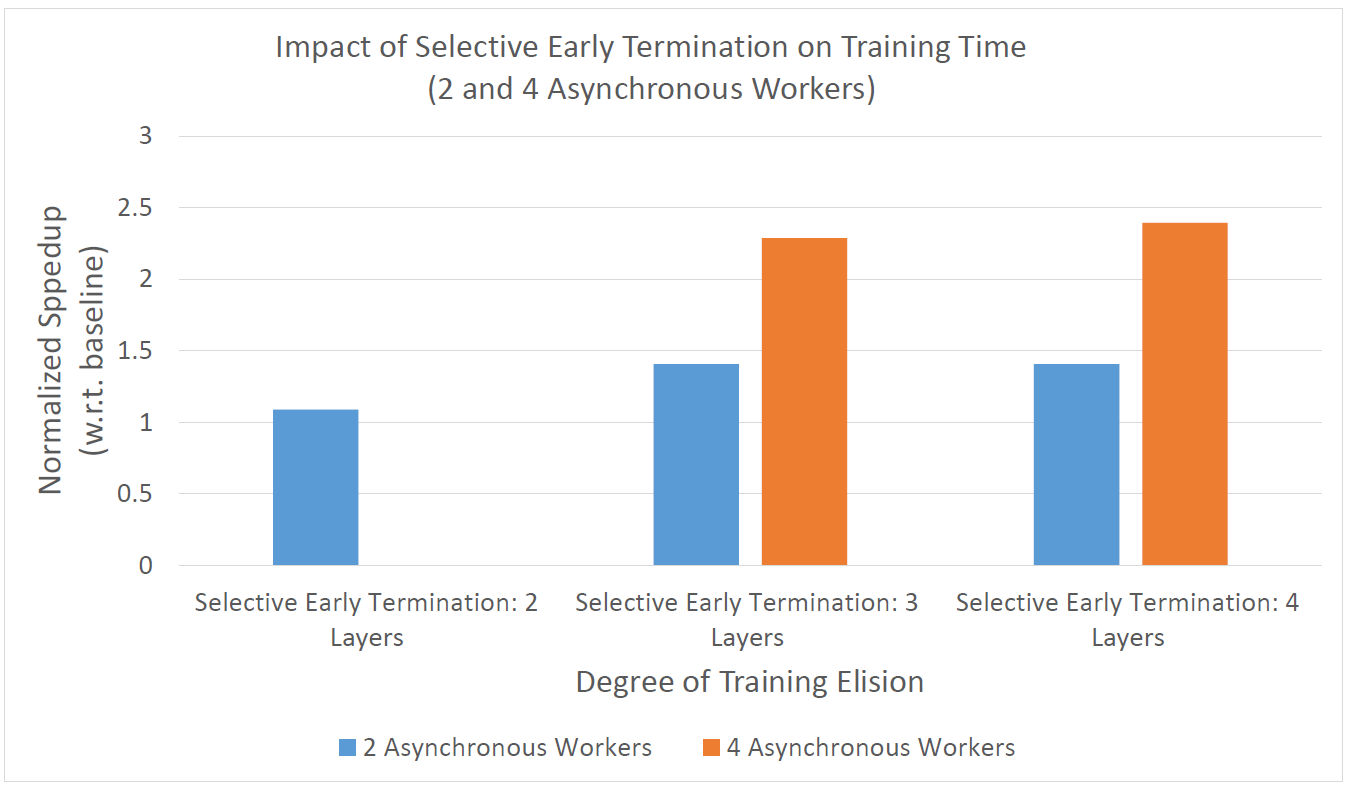
\includegraphics[width=0.8\columnwidth]{figures/fig10.PNG}
	\caption{Normalized speedup for Selective Early Termination: 2 and 4 workers}
	\label{fig:fig10}
\end{figure}
%Figure 8: Selective Early Termination 2 workers (5K steps) -- Accuracy 
%Figure 9: Selective Early Termination 4 workers (2K steps) -- Accuracy
%Figure 10: Selective Early Termination 2 \& 4 (2K \& 5K steps) -- Execution Time

